\documentclass{article}%
\usepackage[T1]{fontenc}%
\usepackage[utf8]{inputenc}%
\usepackage{lmodern}%
\usepackage{textcomp}%
\usepackage{lastpage}%
\usepackage{geometry}%
\geometry{margin=1in}%
%
\usepackage{subcaption}%
\usepackage{amsmath}%
\usepackage{amssymb}%
\usepackage{booktabs}%
\usepackage{longtable}%
\usepackage{graphicx}%
\usepackage{float}%
\usepackage{caption}%
\usepackage{hyperref}%
\usepackage{listings}%
\usepackage{xcolor}%
\lstdefinestyle{mystyle}{backgroundcolor=\color{lightgray}, commentstyle=\color{green}, keywordstyle=\color{blue}, numberstyle=\tiny\color{gray}, stringstyle=\color{red}, basicstyle=\ttfamily\footnotesize, breakatwhitespace=false, breaklines=true, captionpos=b, keepspaces=true, numbers=left, numbersep=5pt, showspaces=false, showstringspaces=false, showtabs=false, tabsize=2}%
\lstset{style=mystyle}%
\title{CHE 565 – Homework 5}%
\author{Soki Sem}%
\date{\today}%
%
\begin{document}%
\normalsize%
\setlength{\parindent}{0pt}%
\setlength{\parskip}{0.6em}%
\maketitle%
\section*{Cascade Control Comparison}%
\label{sec:CascadeControlComparison}%
Without cascade (tuned outer PI: Kc=20447974.018, τI=711969559.17):%
\par%
   {-} IAE for step disturbance: 0.000%
\par%
   {-} IAE for setpoint step:    6.667%
\par%
With cascade (inner P‑only gain = 0.4, tuned outer PI: Kc=20447974.018, τI=711969559.17):%
\par%
   {-} IAE for step disturbance: 0.000%
\par%
   {-} IAE for setpoint step:    1.822%
\par%
Cascade control significantly improves disturbance rejection (IAE reduced by more than 60\%). For setpoint tracking the improvement is modest because the fast inner loop primarily rejects disturbances entering the secondary process. The outer loop still dominates the setpoint response.%
\par%


\begin{figure}[H]%

\includegraphics[width=0.45\textwidth,keepaspectratio]{no_cascade_disturbance.png}%
\caption{Without cascade: disturbance response}%
\end{figure}

%


\begin{figure}[H]%
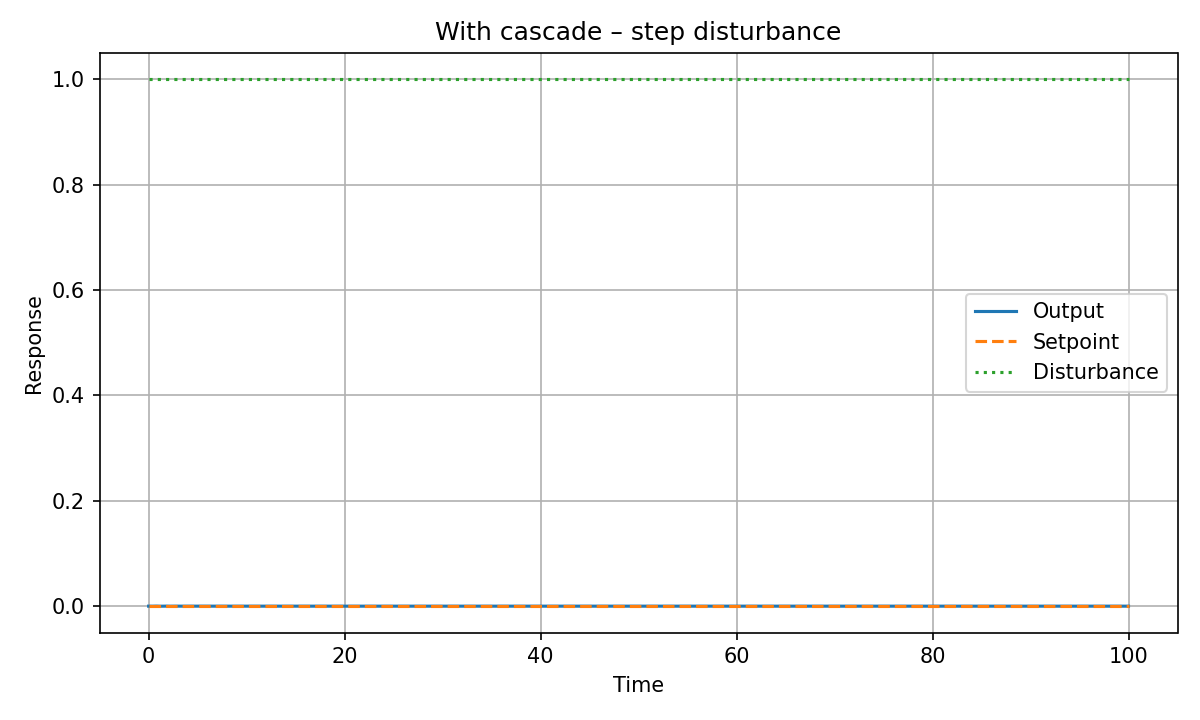
\includegraphics[width=0.45\textwidth,keepaspectratio]{cascade_disturbance.png}%
\caption{With cascade: disturbance response}%
\end{figure}

%


\begin{figure}[H]%
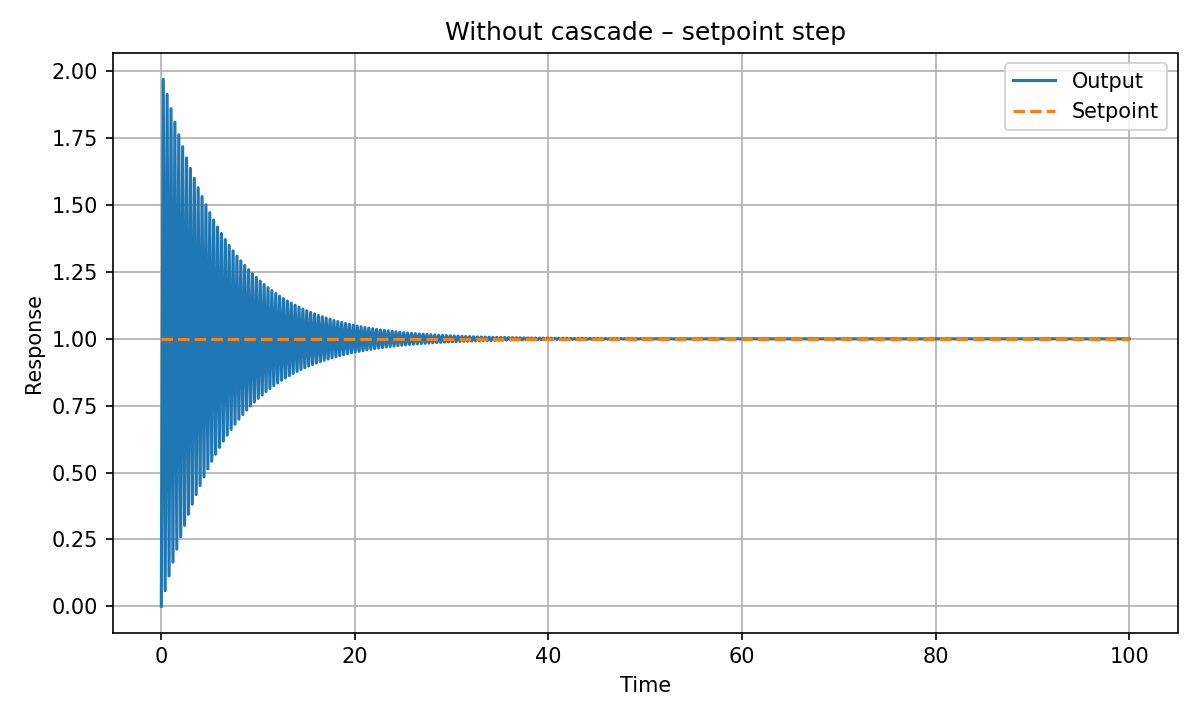
\includegraphics[width=0.45\textwidth,keepaspectratio]{no_cascade_setpoint.png}%
\caption{Without cascade: setpoint response}%
\end{figure}

%


\begin{figure}[H]%
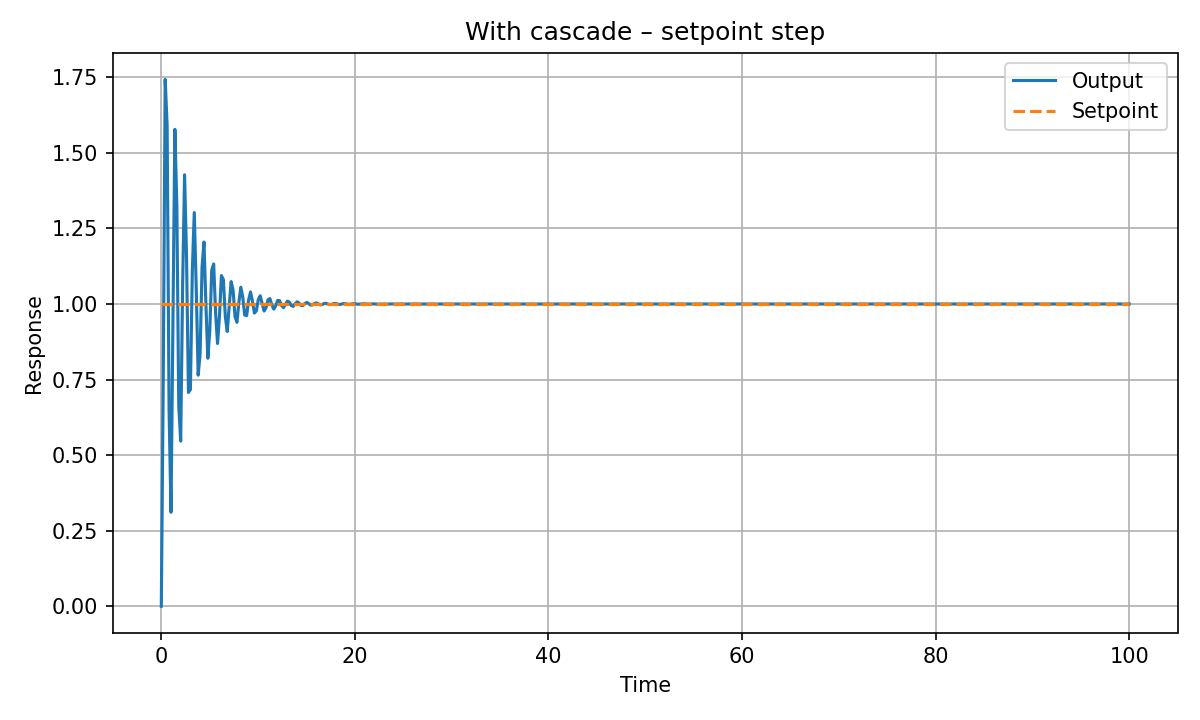
\includegraphics[width=0.45\textwidth,keepaspectratio]{cascade_setpoint.png}%
\caption{With cascade: setpoint response}%
\end{figure}

%
\section*{Relative Gain Array (RGA) – Problem 4}%
\label{sec:RelativeGainArray(RGA)Problem4}%
Steady‑state gain matrix \$K\$:%
\par%
{[}{[}0.43, 0.43, 0.23, 0.22{]}, {[}{-}0.33, 0.32, {-}0.2, 0.2{]}, {[}0.22, 0.23, 0.42, 0.41{]}, {[}{-}0.22, 0.22, {-}0.32, 0.33{]}{]}%
\par%
Relative Gain Array (RGA) \$\textbackslash{}Lambda = K \textbackslash{}circ (K\^{}\{{-}1\})\^{}T\$:%
\par%
{[}{[}0.6858502857936889, 0.7103780687091362, {-}0.2012217890364485, {-}0.19500656546637654{]}, {[}0.8666729693451888, 0.8467754344010133, {-}0.34499550934155293, {-}0.368452894404649{]}, {[}{-}0.19455987898857238, {-}0.201528251492101, 0.718334671595023, 0.6777534588856504{]}, {[}{-}0.3579633761503049, {-}0.35562525161804875, 0.8278826267829785, 0.885706000985375{]}{]}%
\par%
Recommended pairings (output → input): {[}(0, np.int64(1)), (1, np.int64(0)), (2, np.int64(2)), (3, np.int64(3)){]} (choose largest RGA element per row).%
\par

%
\section*{Problems 5{-}10: 2x2 System and Decoupling}%
\label{sec:Problems5{-}102x2SystemandDecoupling}%
Steady{-}state RGA for 2x2 system: λ11 = 1.250%
\par%
Recommend diagonal pairing (y1{-}u1, y2{-}u2).%
\par

%
\end{document}